
\begin{table}[htbp]
  \caption{递签简表}
  \centering
  \begin{tabular}{r|l}
    \toprule
    地点 & 亮马桥外交大楼 {\color{blue} D1 座 1302}【而非邮件里说的 E 座】 \\ \midrule
    流程 & 8:00 -- 9:00 取号、填写 EMS 邮寄单、整理比对递签材料 \\
    & 9:00 -- 12:00 逐一递签(我们这次时间延长到 12:30 左右。会保证每人至少一次递签机会) \\
    \bottomrule
  \end{tabular}
\end{table}
% 1.地点:亮马桥外交大楼 DI 座 1302【而非邮件里说的 E 座】 

% 2.虽然预约的时间是8:00-9:00,但其实九点才开始受理。但还是建议早点去,因为可以早点上去取号,取了号再下楼办EMS的邮寄单。这样可以防止取到的号比较靠后。 

% 3.等待的地方是一间小屋子,墙上有申请表的填写模板和递交材料的顺序,可以对照看自己的填写和材料的顺序。 

% 4.【等待的小屋子不许玩手机,不许用电脑,不许用电子设备。建议自备其他休闲娱乐方式】 

\section{材料顺序及 APS 模板}
\begin{figure}[htbp]
  \centering
  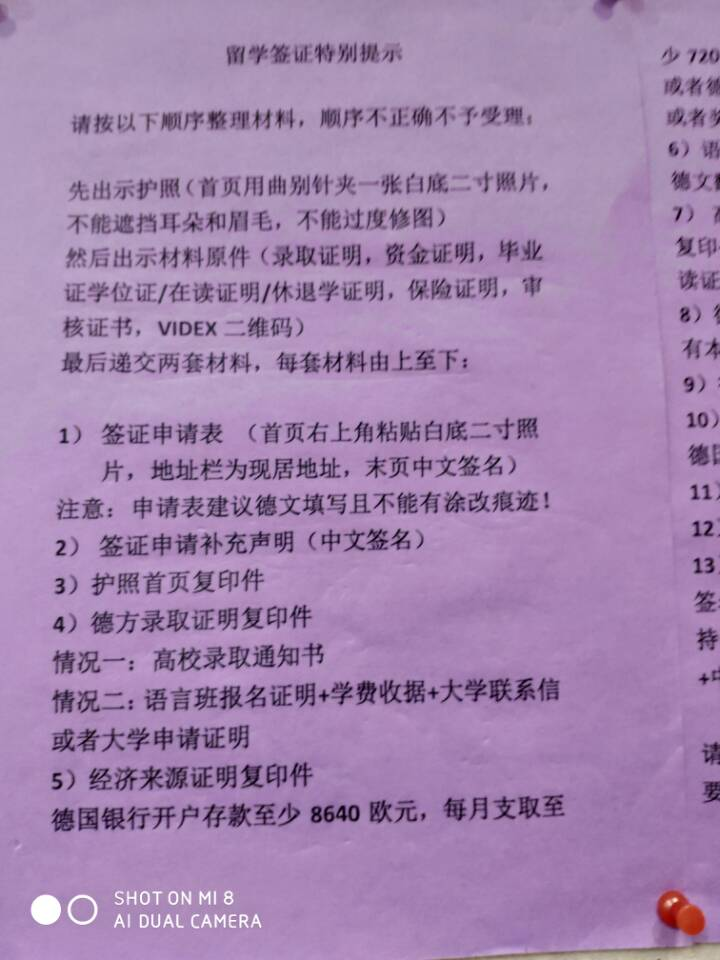
\includegraphics[width=\textwidth]{order-1}
  \caption{材料顺序要求第 1 页。摄于 2019 年 1 月 17 日}
  \label{fig:order-1}
\end{figure}
\begin{figure}[htbp]
  \centering
  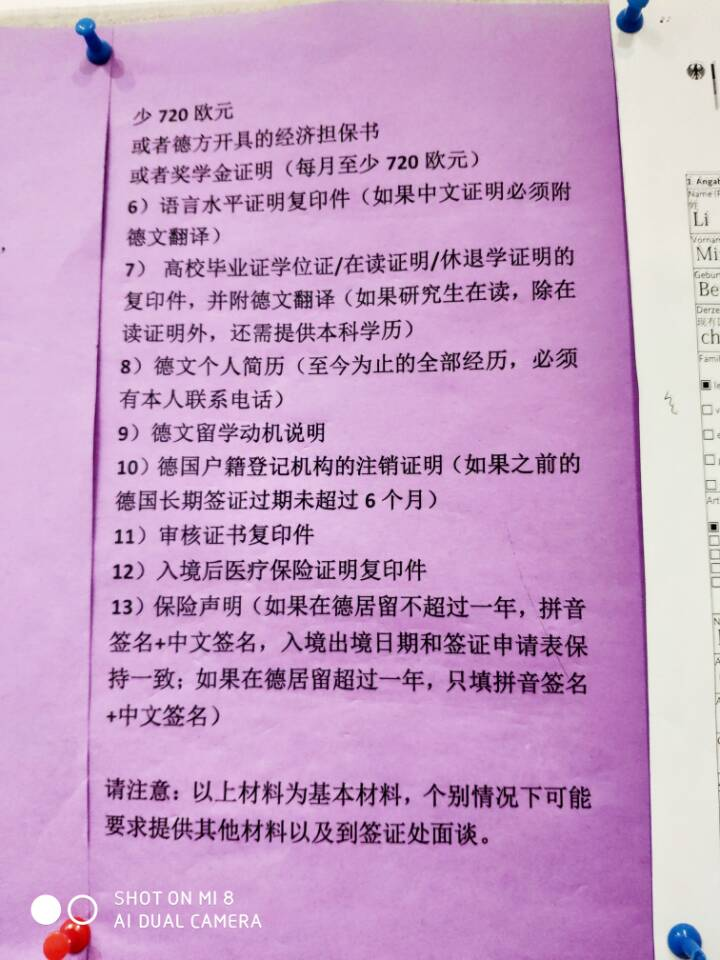
\includegraphics[width=\textwidth]{order-2}
  \caption{材料顺序要求第 2 页。摄于 2019 年 1 月 17 日}
  \label{fig:order-2}
\end{figure}
\begin{figure}[htbp]
  \centering
  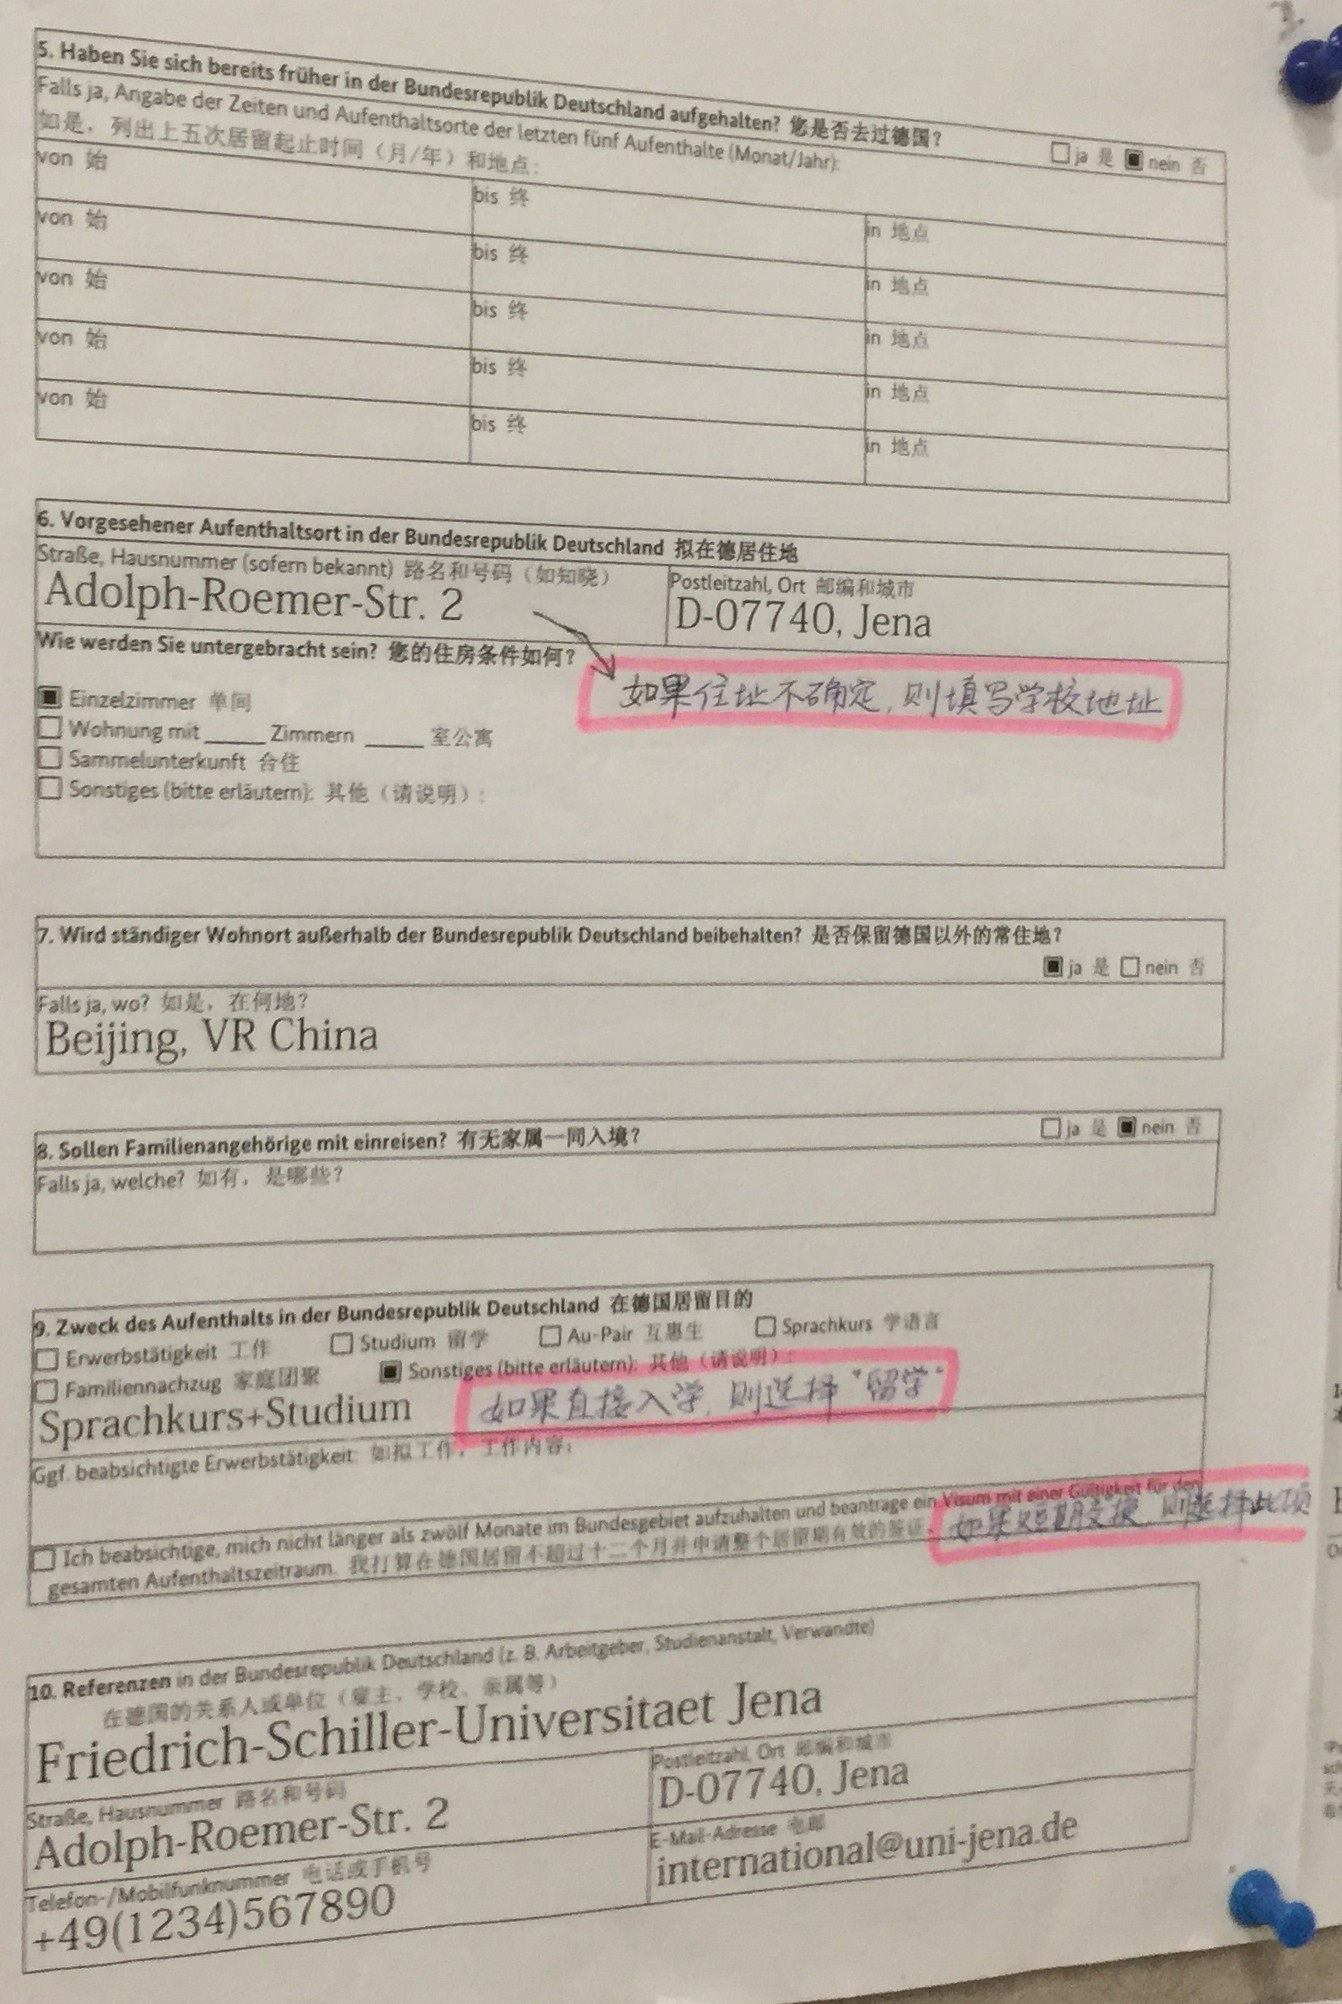
\includegraphics[width=\textwidth]{APS-forms}
  \caption{APS 申请表填写模板。摄于 2019 年 1 月 17 日}
  \label{fig:APS-forms}
\end{figure}

\section{路线图}
\begin{figure}[htbp]
  \centering
  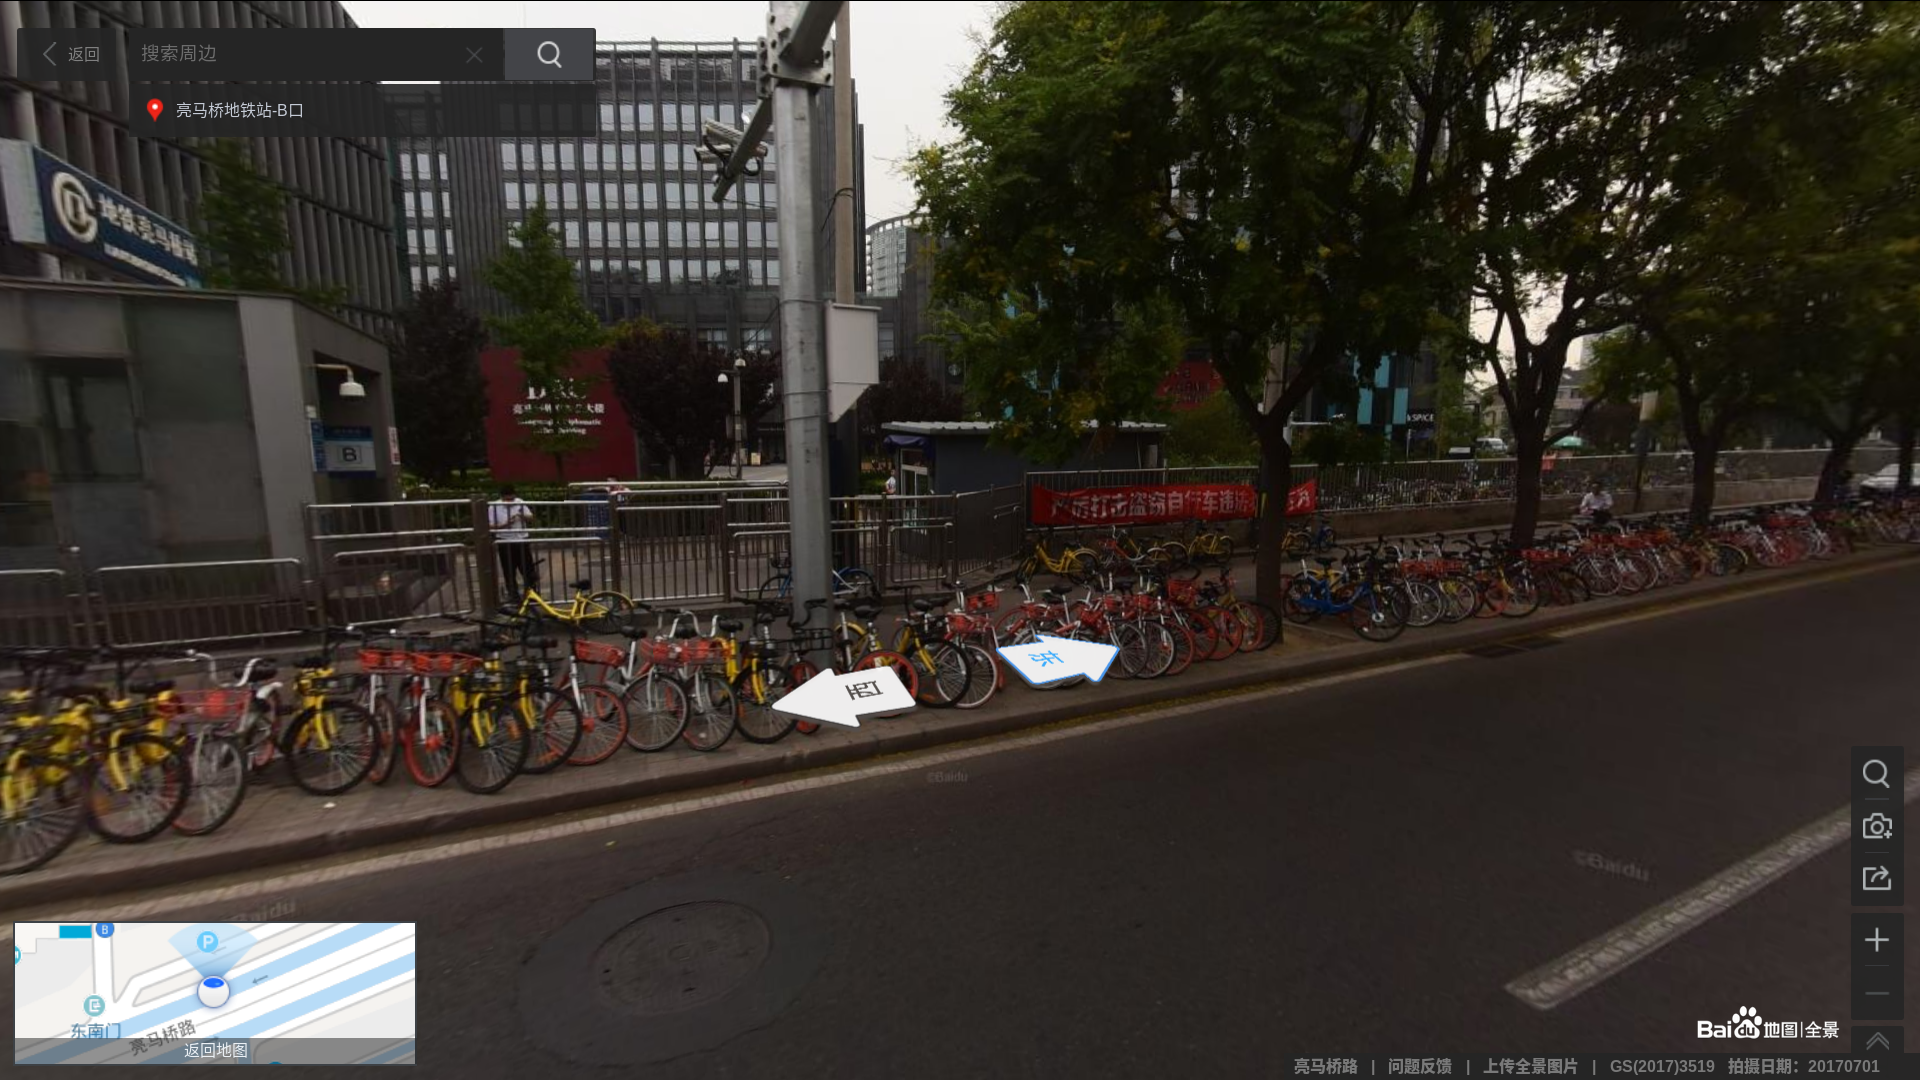
\includegraphics[width=\linewidth]{metro-B}
  \caption[亮马桥地铁 B 口]{亮马桥地铁 B 口。截图来自 \href{https://map.baidu.com/\#panoid=09002200121707010630058282I\&panotype=street\&heading=0.64\&pitch=-4.92\&l=19\&tn=B_NORMAL_MAP\&sc=0\&newmap=1\&shareurl=1\&pid=09002200121707010630058282I}{百度全景}。}
  \label{fig:real}
\end{figure}
\begin{figure}
  \centering
  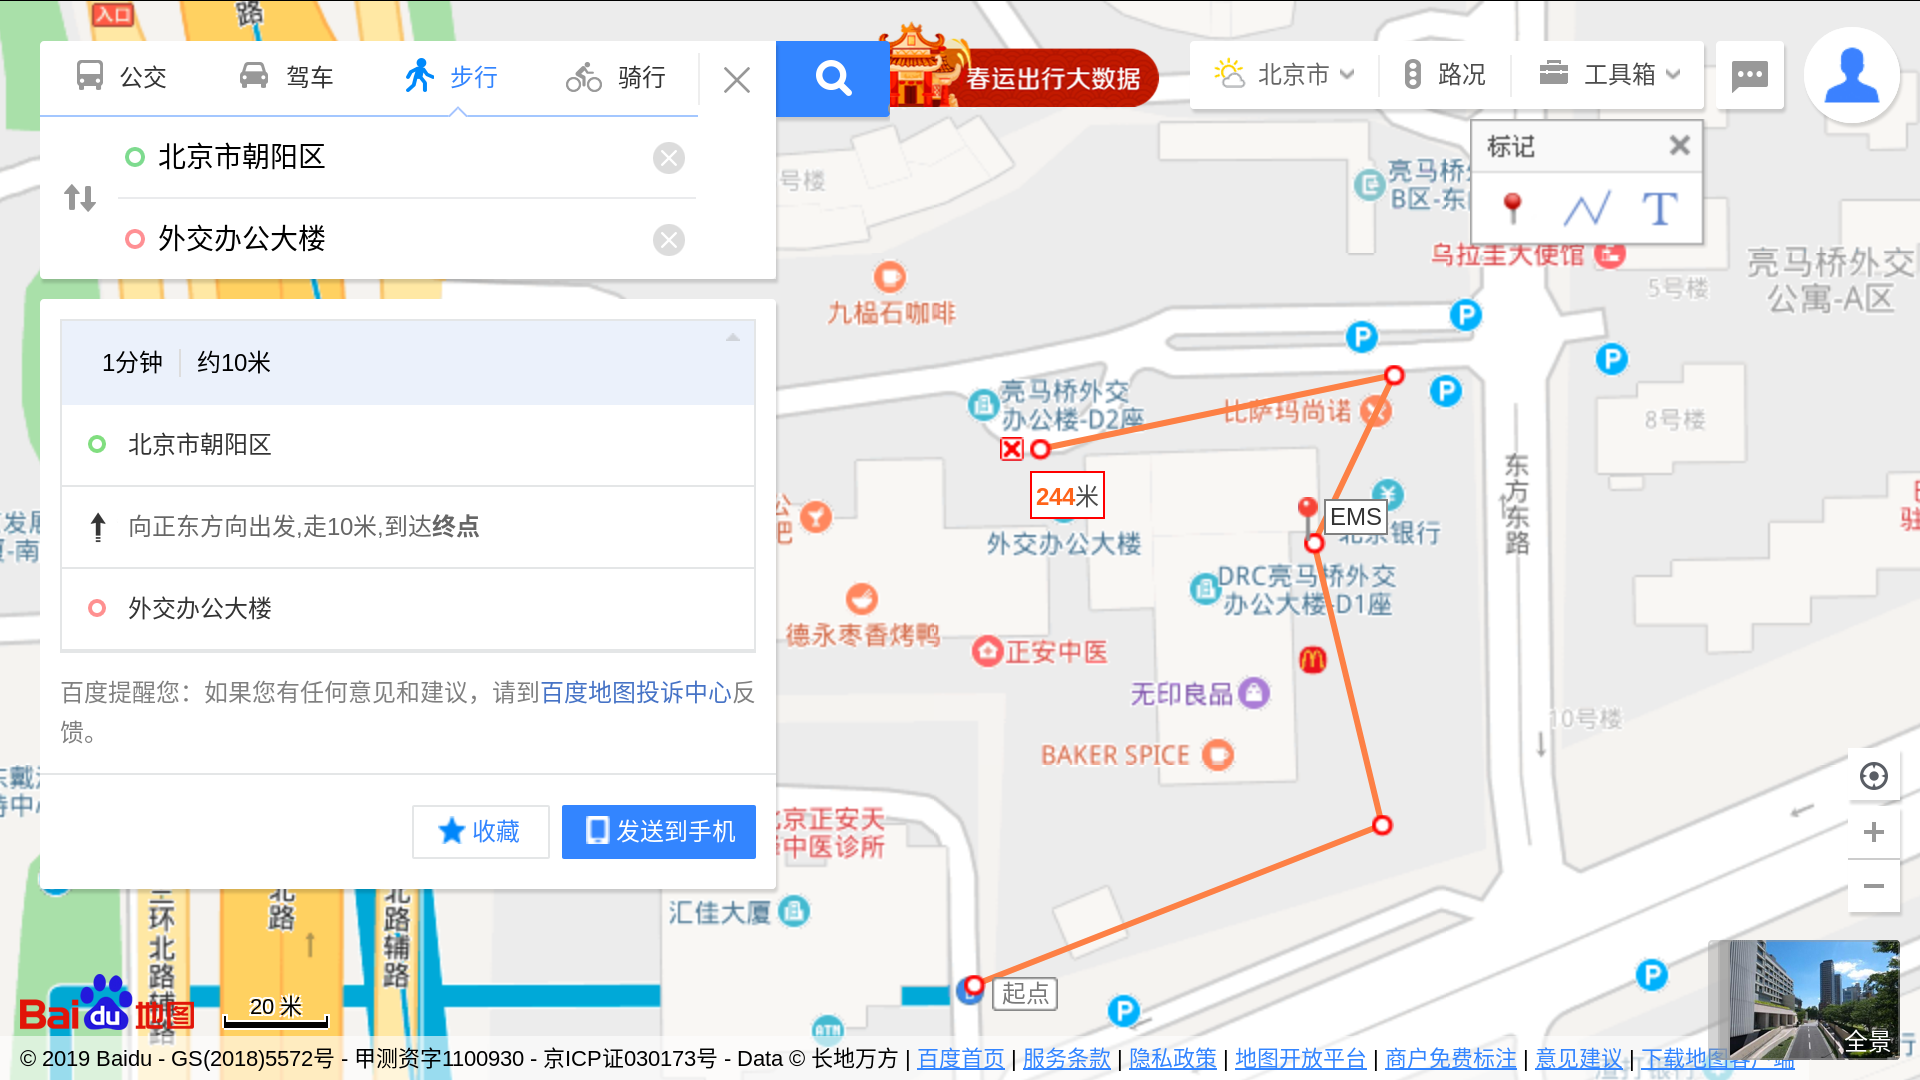
\includegraphics[width=\linewidth]{route-to-D1}
  \caption[地铁 B 口前往 D1 座路线]{地铁 B 口前往 D1 座路线。路经 EMS. 截图来自\href{https://map.baidu.com/}{百度地图}。}
  \label{fig:route}
\end{figure}
\begin{figure}
  \centering
  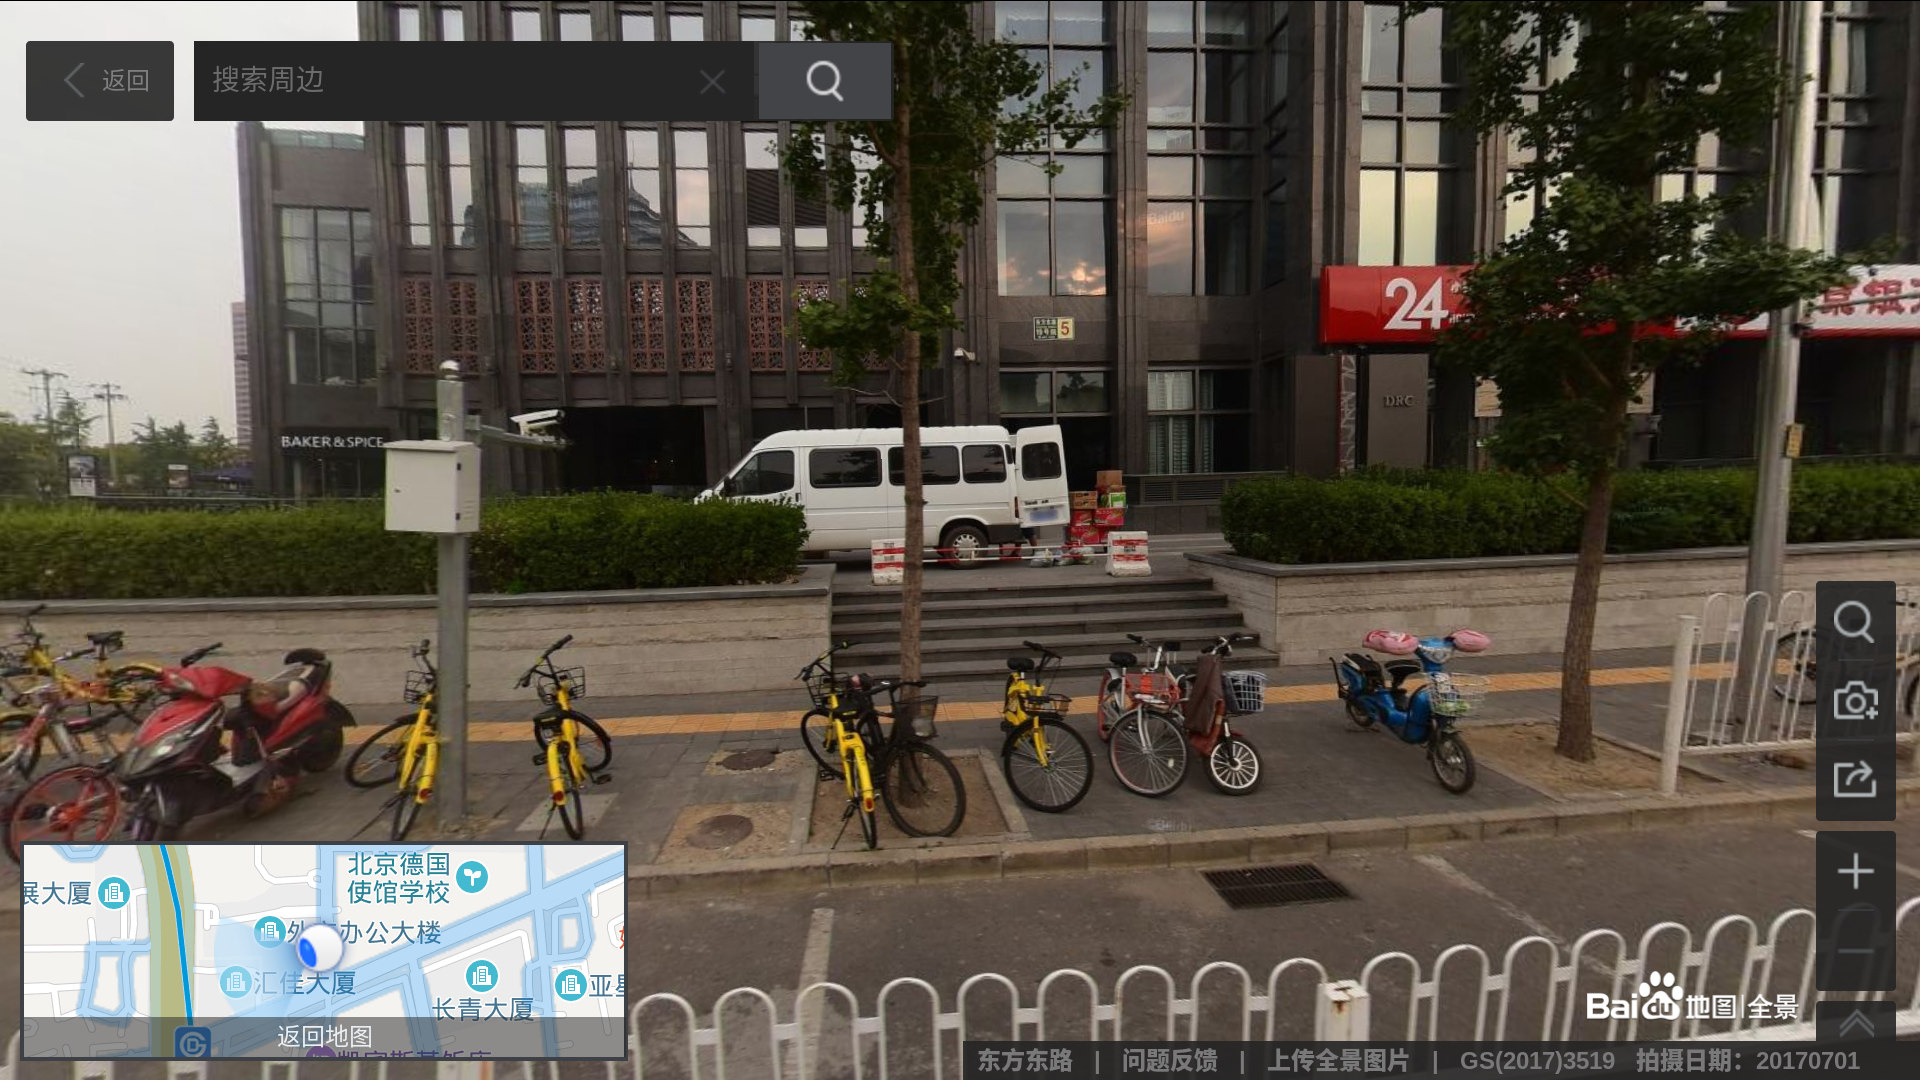
\includegraphics[width=\linewidth]{EMS}
  \caption[EMS 办理处]{EMS 办理处。应该是在图中汽车的后面,并从车的左侧进入通道。截图来自\href{https://map.baidu.com/\#panoid=09002200121707010635276742I\&panotype=street\&heading=274.99\&pitch=-2.29\&l=12\&tn=B_NORMAL_MAP\&sc=0\&newmap=1\&shareurl=1\&pid=09002200121707010635276742I}{百度地图}。我当时忘了拍照。抱歉。}
  \label{fig:EMS}
\end{figure}